\documentclass[12pt,parskip=full]{scrartcl}
\usepackage[utf8]{inputenc}   % UTF8-Kodierung für Umlaute
\usepackage{ngerman}          % deutsche Silbentrennung
\usepackage[T1]{fontenc}	  % wichtig für Trennung von Wörtern mit Umlauten
\usepackage{microtype}		  % verbesserter Randausgleich
\usepackage{graphicx}         % Einbindung von Grafiken
\usepackage{wrapfig}			% Grafiken im Text

\title{Ausführliche Nähanleitung Mund-Nasen-Schutz mit Nackenband}
\author{Anna Klingauf}
\date{Oktober 2020}

\begin{document}
\begin{titlepage}
\maketitle
\thispagestyle{empty}
\begin{figure}[b!] 
  \centering
     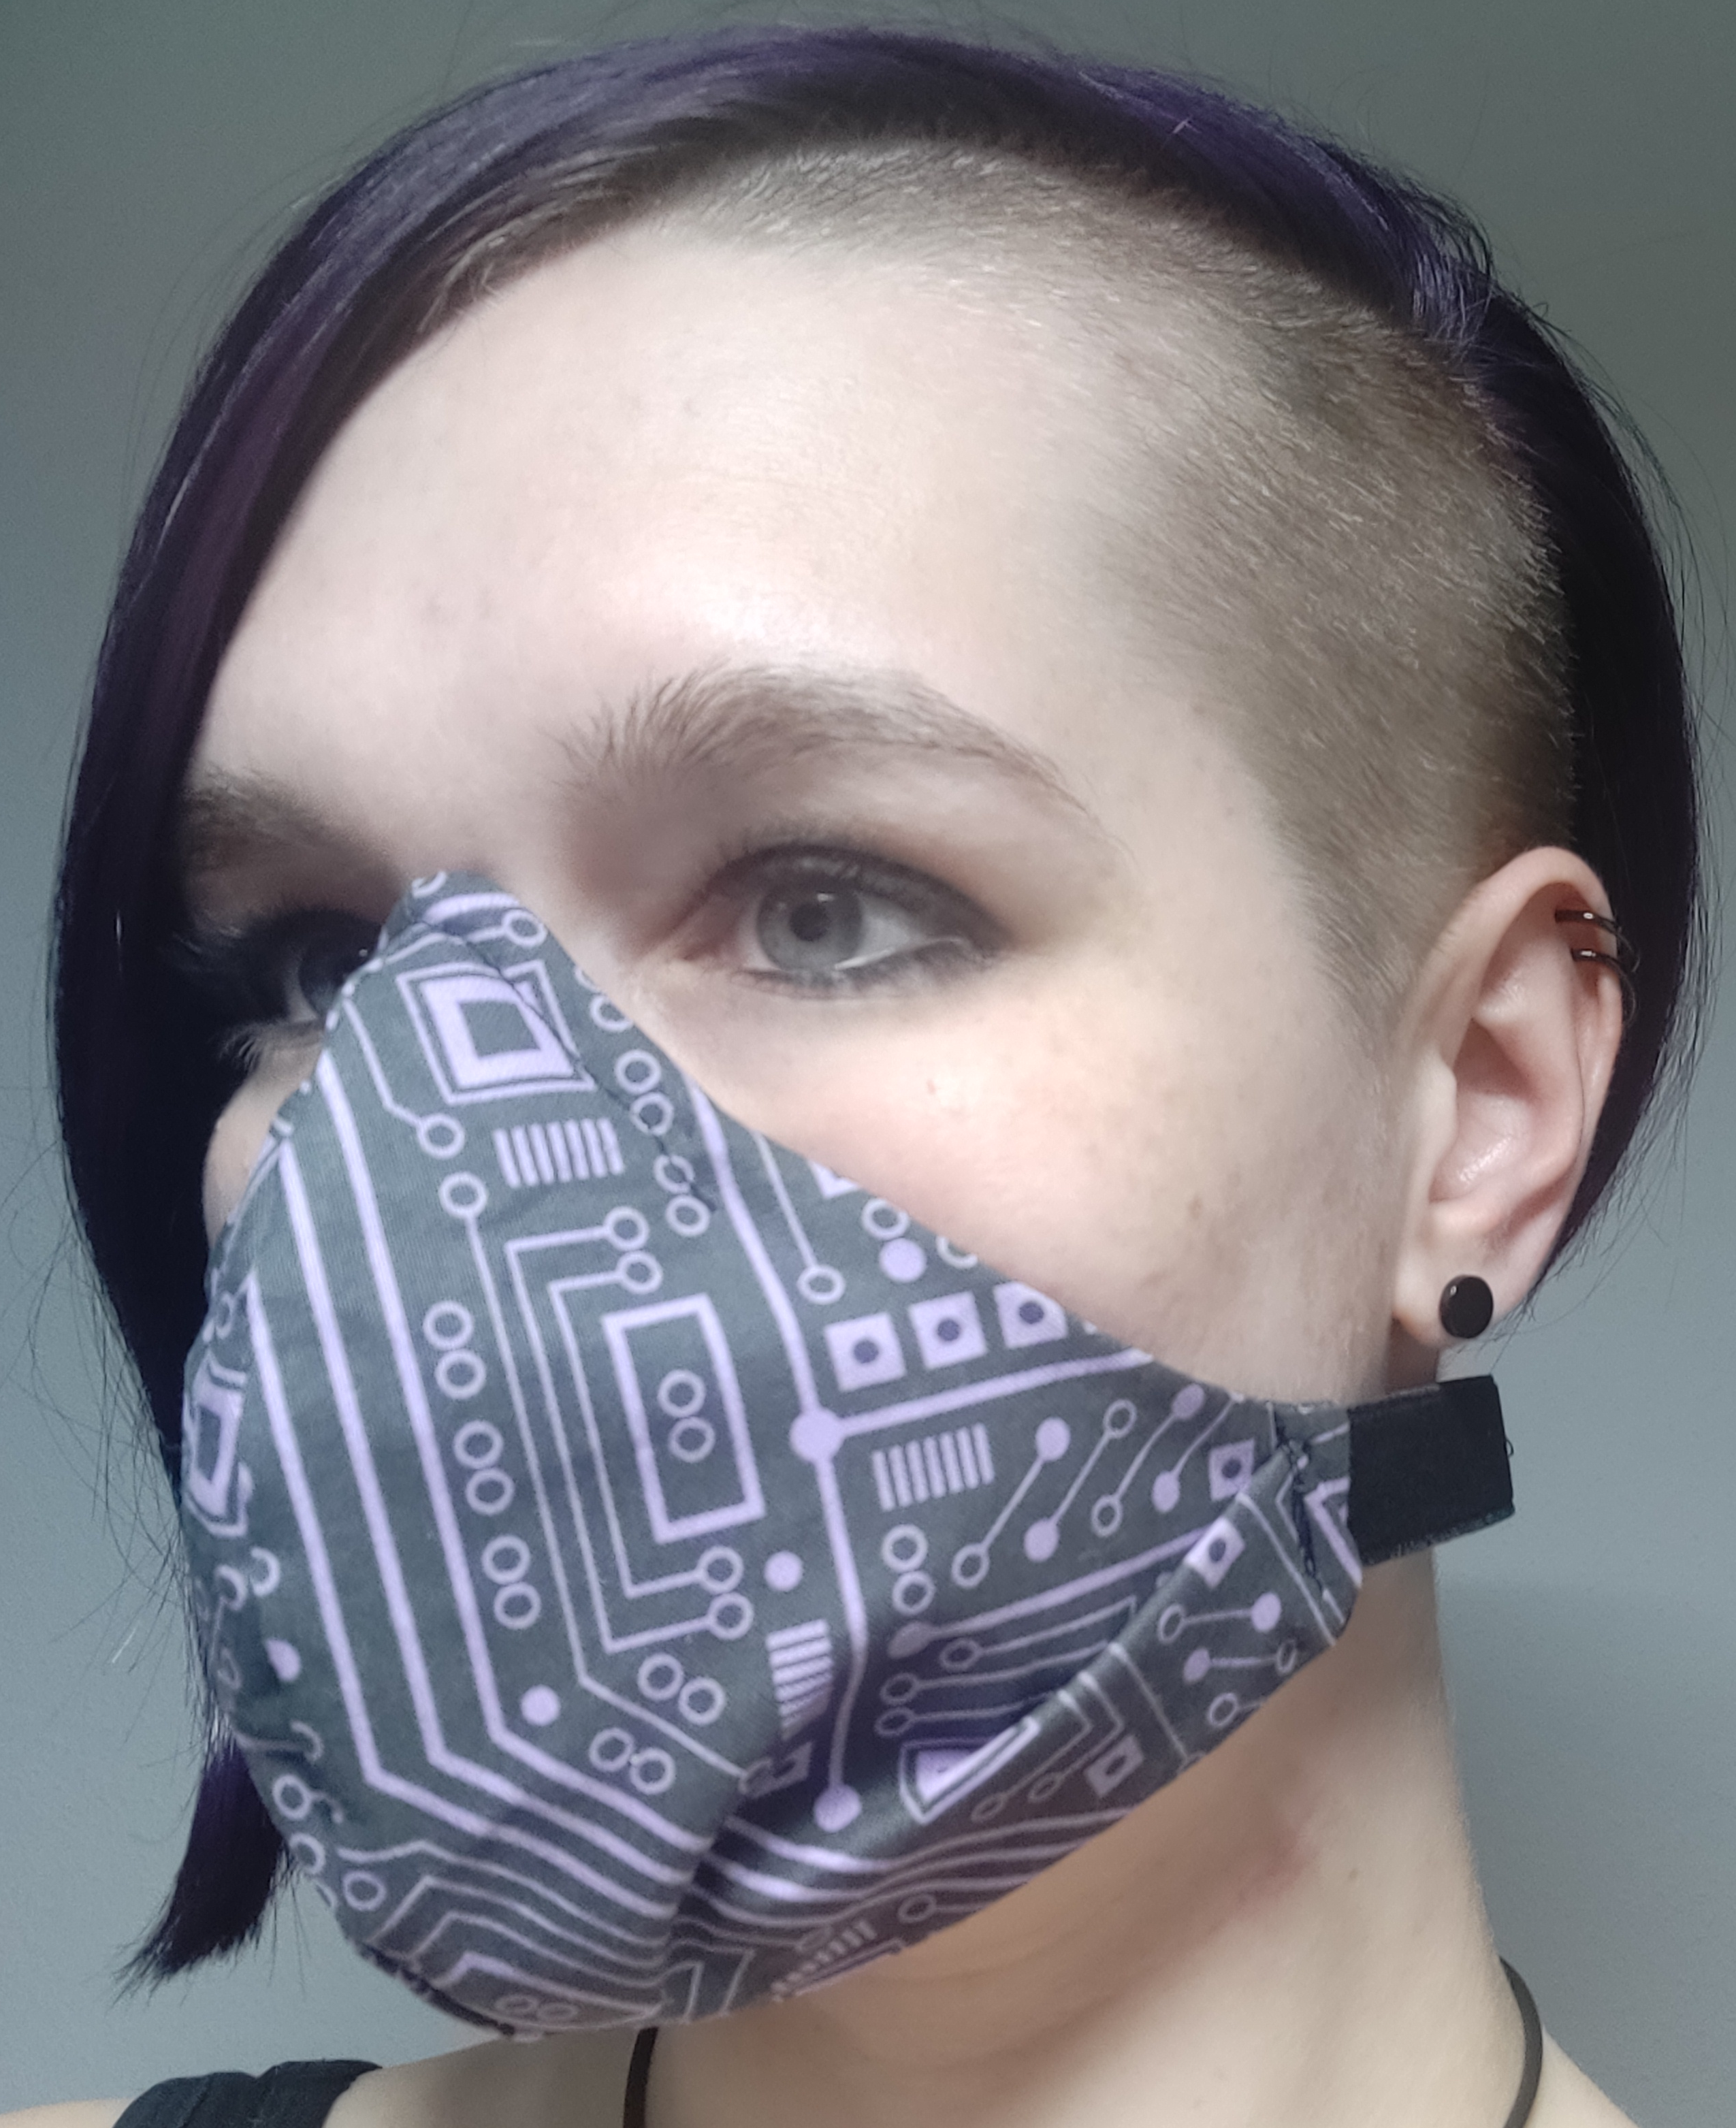
\includegraphics[width=0.60\textwidth]{Bilder/Fertig/Gesamt.png}
\end{figure}
\end{titlepage}
\clearpage

\section{Allgemeines}
Der Mund-Nasen-Schutz (abgekürzt MNS oder Maske) wie er hier vorgestellt wird besteht aus zwei Lagen Baumwollstoff. Im Gegensatz zu den meisten anderen MNS wird er nicht an den Ohren befestigt sondern mit einem elastischen Band im Nacken. Das Band kann mit Klett, Knöpfen oder Druckknöpfen geschlossen werden. An der Nase ist sowohl ein Drahteinsatz als auch eine Abdichtung mit Gummi angebracht. Da die Maske durch die Form und die Abdichtung an der Nase sehr dicht ist, beschlägt bei allen bisherigen Testpersonen die Brille nicht. Die Faltung der Maske kann beim Nähen individuell an das Gesicht angepasst werden. Es werden drei Größen als Vorschläge zur Verfügung gestellt, die auch individuell angepasst werden können.

\section{Materialien}
Folgende Materialien werden benötigt:



\end{document}
